\section{ Filler lecture:Exoplanets }\label{sec:q5}    


\subsection*{a)}
From observation, the short periodic function has a period of ~0.05 year (planet 1), whilst the long periodic function has a period of ~0.7 year (planet 2). We can then calculate the radius of each orbit as follows:

\begin{equation}
\begin{split}
    T = 2 \pi \sqrt{ \frac{r^3}{GM}} \\
    r_{orbit} = \sqrt[3]{GM \left(\frac{T}{2 \pi} \right)^2 }
\end{split}
\end{equation}

And so we get:
\begin{equation*}
\begin{split}
    r_1 = \sqrt[3]{6.674E-11 \cdot 2E30 \cdot \left(\frac{0.05\cdot365.25\cdot24\cdot60^2}{2 \pi} \right)^2 } = 2.03E10 \; m = 0.135 \; AU \\
    r_2 = \sqrt[3]{6.674E-11 \cdot 2E30 \cdot \left(\frac{0.7\cdot365.25\cdot24\cdot60^2}{2 \pi} \right)^2 } = 1.18E11 \; m = 0.786 \; AU \\
\end{split}
\end{equation*}
We now assume that since the observer is far away, the star and the planet are effectively flat discs, and the reduction in stellar flux is directly proportional to the reduction in area from the planet moving in front of the star. Further, we will indicate the reduced flux, as measured in the data, by $\phi_r$. This means that:

\begin{equation}
\begin{split}
    \frac{A_{star} - A_{planet}}{A_{star}} = \phi_r \\
    A_{planet} = 2 \pi r_{planet}^2 = A_{star} (1-\phi_r) \\
    r_{planet} = \sqrt{ \frac{A_{star} (1-\phi_r)}{2\pi}} \\
\end{split}
\end{equation}

Which leads to:

\begin{equation}
\begin{split}
    r_{1} = \sqrt{ \frac{2 \pi \cdot (7E8)^2 (1-0.990)}{2\pi}} = 7.00E7 \; m\\
    r_{2} = \sqrt{ \frac{2 \pi \cdot (7E8)^2 (1-0.994)}{2\pi}} = 5.42E7 \; m\\
\end{split}
\end{equation}

\subsection*{b1)}
\begin{enumerate}
    \item Radial Velocity Method
    \item Gravitational Micro-lensing
    \item Timing method
\end{enumerate}

\subsection*{b2)}
\begin{enumerate}
    \item Mass, period
    \item Mass, period
\end{enumerate}
\subsection*{b3)}
\begin{enumerate}
    \item High masses
    \item High masses
\end{enumerate}
\subsection*{c)}

\subsection*{d)}

The question is  rather non-specific as to the nature of this tail, so we will make some assumptions first:
\begin{enumerate}
    \item The tail is completely opaque
    \item The tail remains the same size and remains opaque for at least the transfer time.
\end{enumerate}
This will cause a band to form across the star with left-behind planetary matter to blot out the star partially. This is illustrated in the figure too. We approximate the area of this band by a rectangle, ignoring the curvature of the sun at the edges. Once the planet has completed the full transfer, and the band crosses the whole sun, the area reduction is:

\begin{equation}
    \frac{A_star-2r_{star}\cdot 2 r_{planet}}{A_star} = \frac{2\pi \cdot (7E8)^2 - 2\cdot (7E7)\cdot 2 (7E8)}{2\pi \cdot (7E8)^2} = 0.936.
\end{equation}

This results in the curve found in the figure. First, the planet enters the scene, reducing the stellar flux by 1\%, but gradually the flux reduces further, as the band passes over the star. At the end of the transfer at ~250 minutes, only 93.6\% of the light is left, but then it stops reducing. 

\begin{figure}[H]
    \centering
    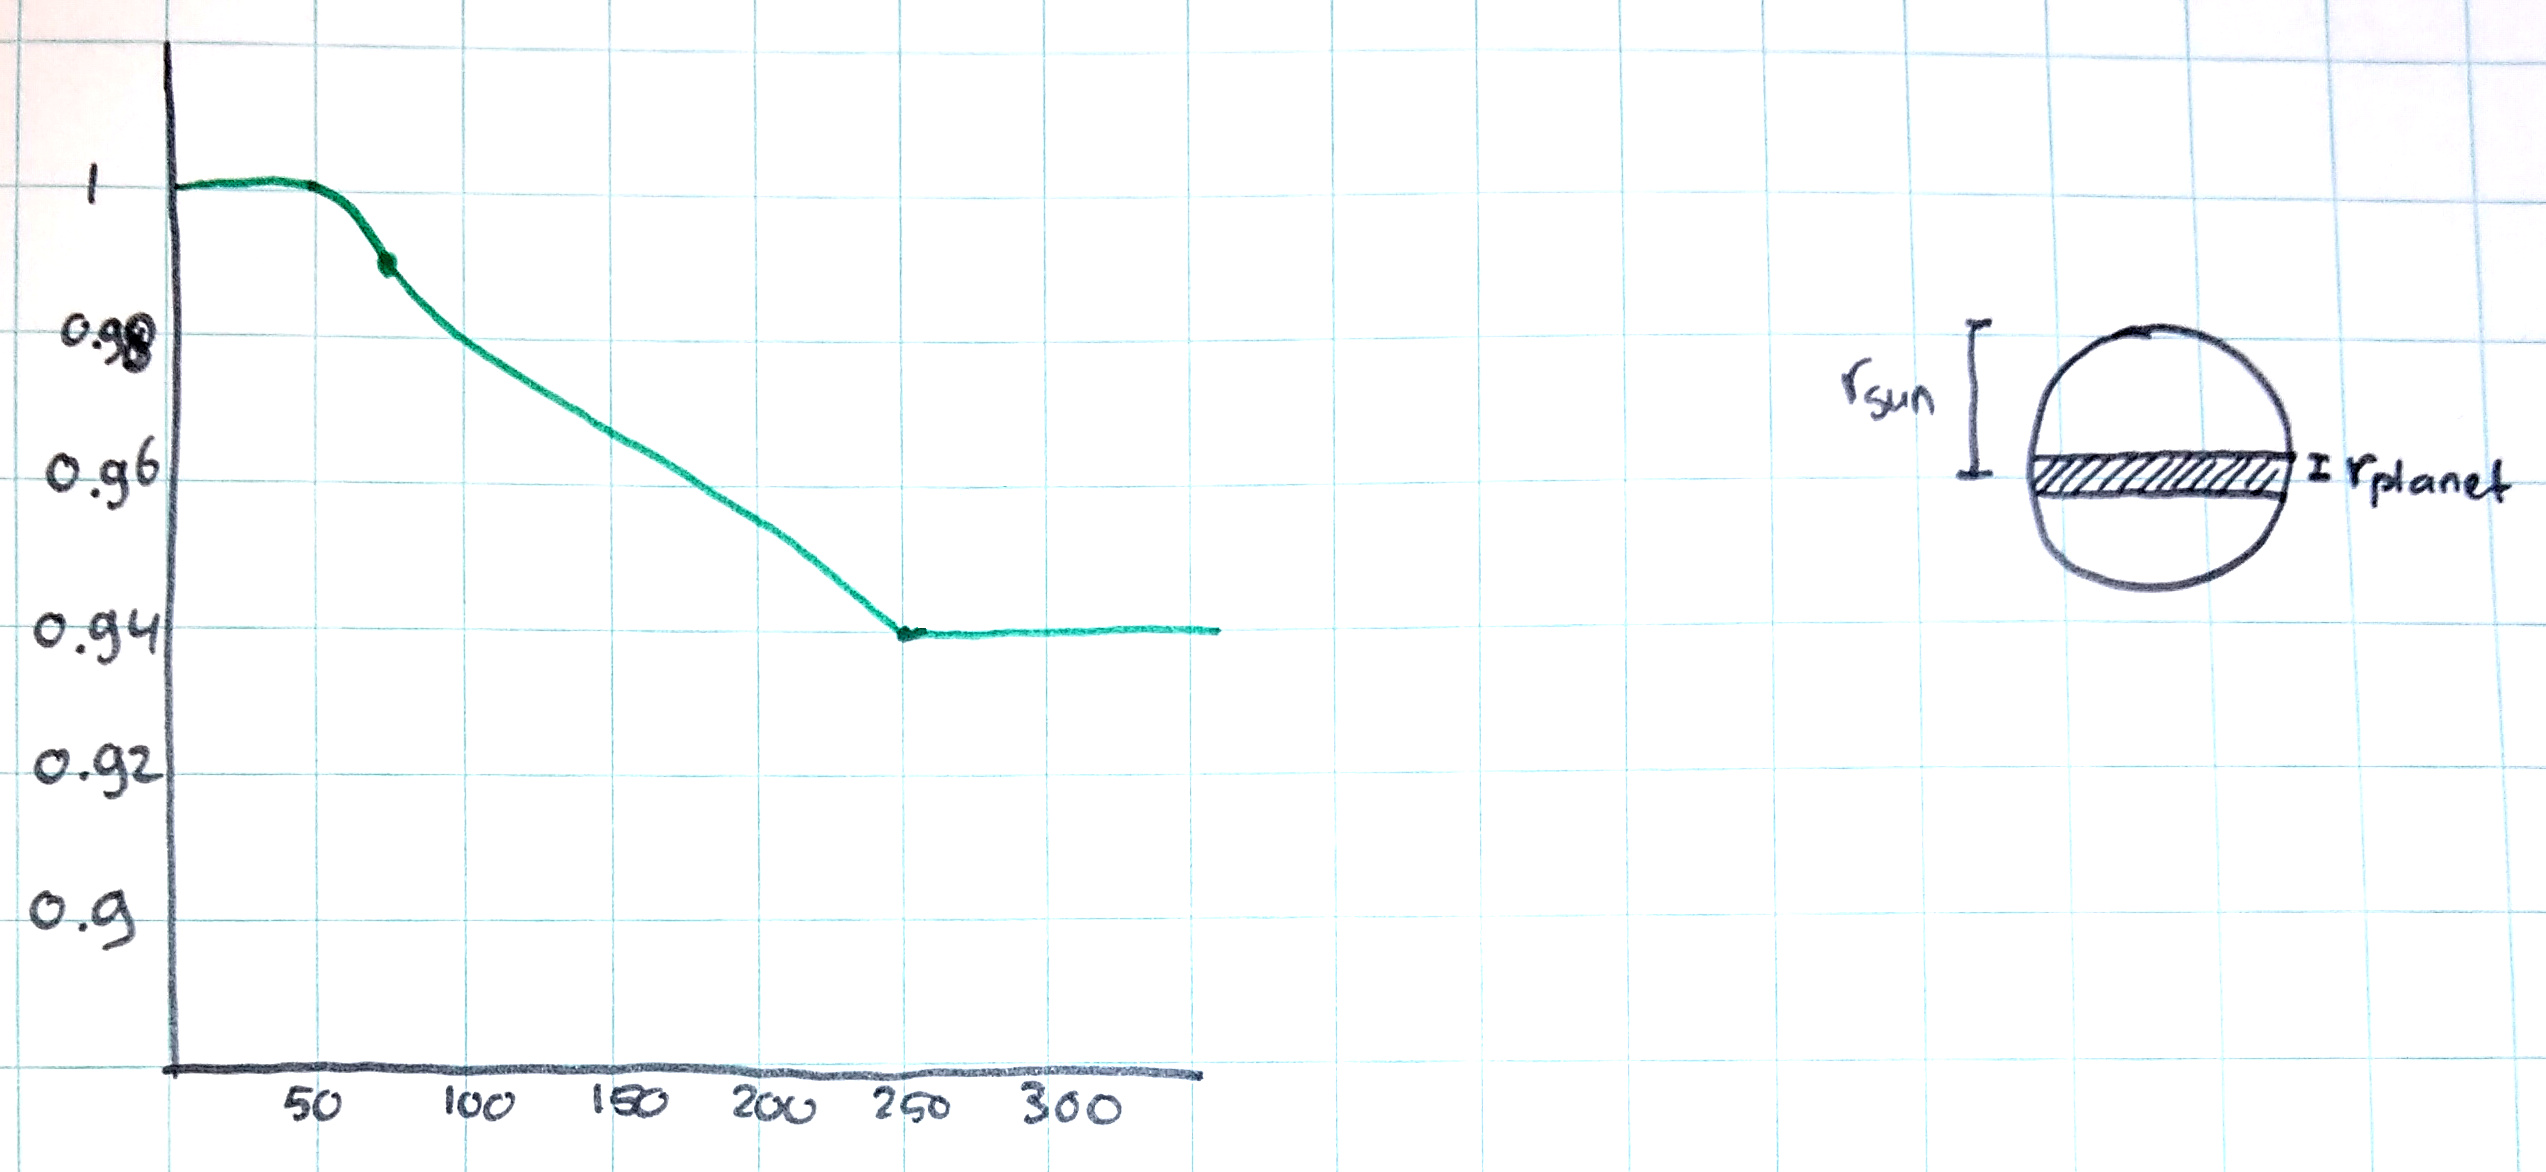
\includegraphics[width=0.9\textwidth]{figures/5d.jpg}
    %\caption{Caption}
    \label{fig:my_label5}
\end{figure}
